\usepackage{hyperref}

\section{Redes de Petri}

\subsection{IOPT-Tools}

\subsubsection{Rede de Petri --- Tapete Singular}
\begin{figure}[H]
    \centering
    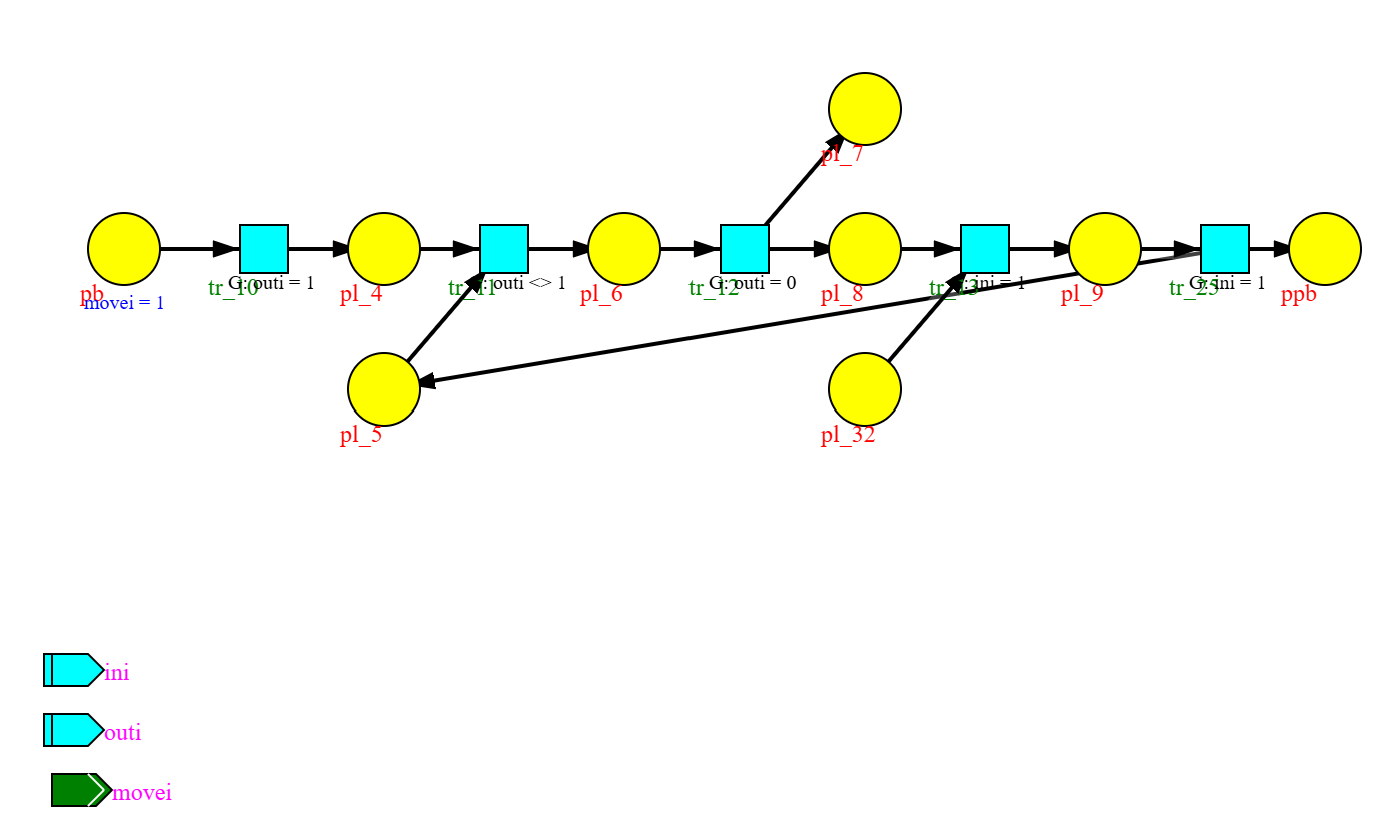
\includegraphics[width=0.8\textwidth]{img/petri_tapete_singular.png}
    \caption{Rede de Petri --- Tapete Singular}\label{fig:petri_tapete_singular}
\end{figure}

\subsubsection{Rede de Petri --- Modelo Completo}
\begin{figure}[H]
    \centering
    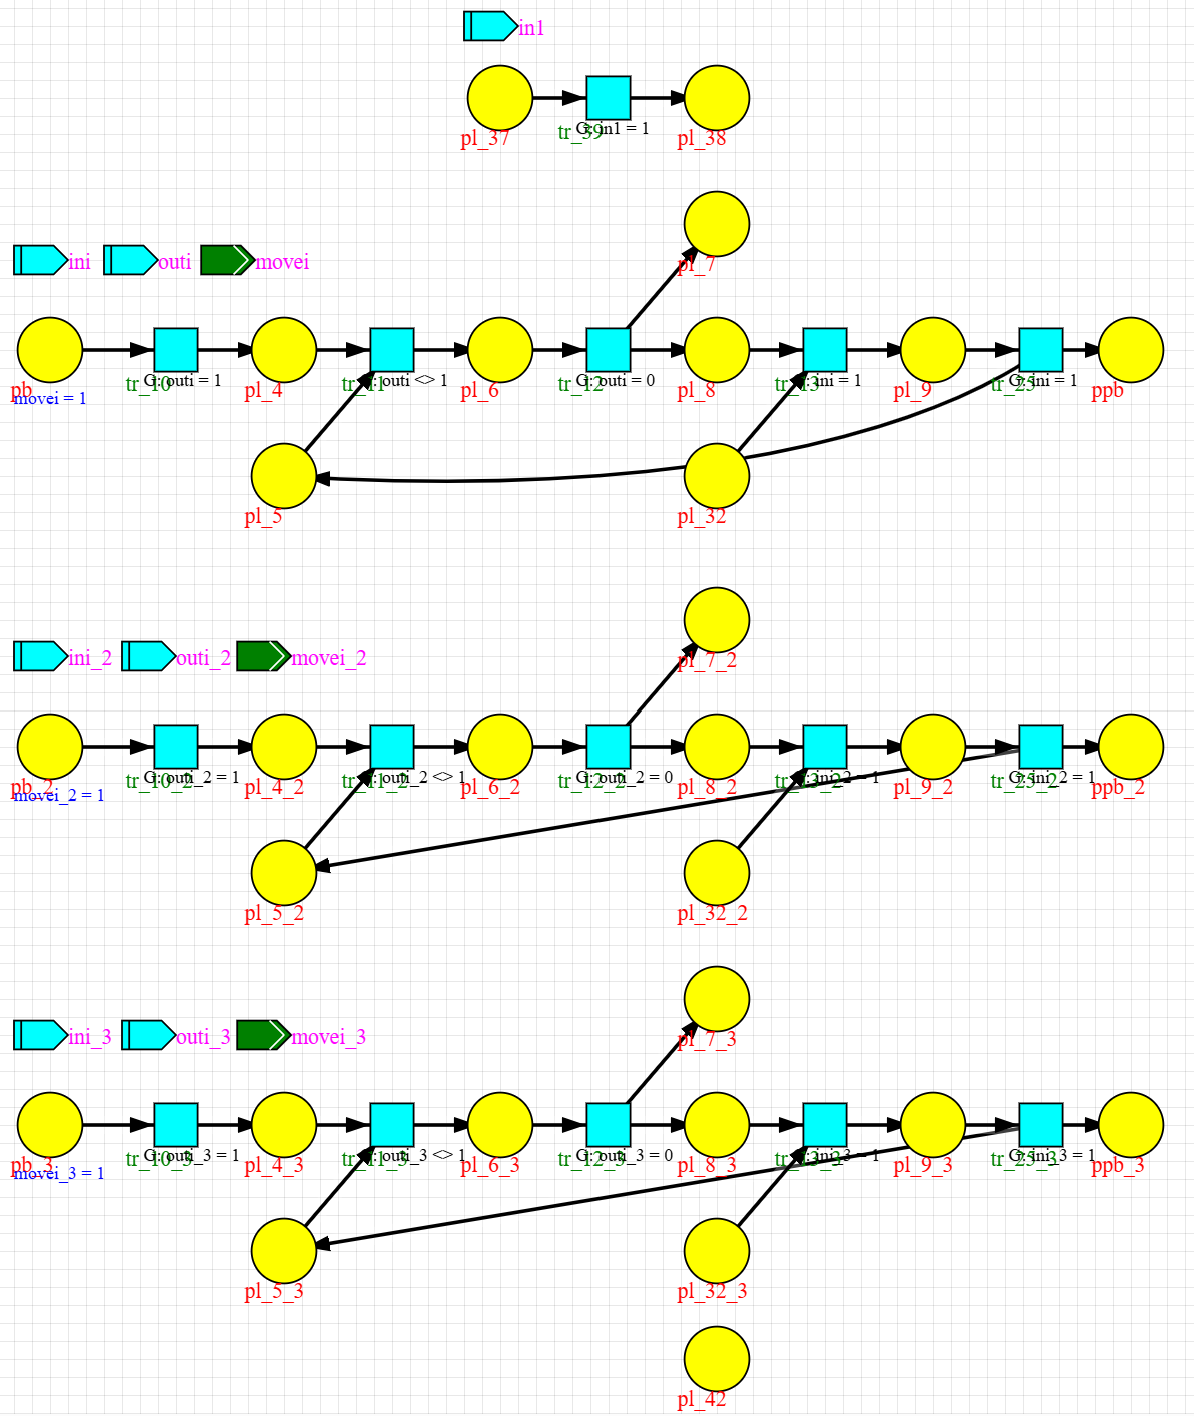
\includegraphics[width=0.8\textwidth]{img/petri_modelo_completo.png}
    \caption{Rede de Petri --- Modelo Completo}\label{fig:petri_modelo_completo}
\end{figure}

\subsubsection{Rede de Petri --- Fusion set}
\begin{figure}[H]
    \centering
    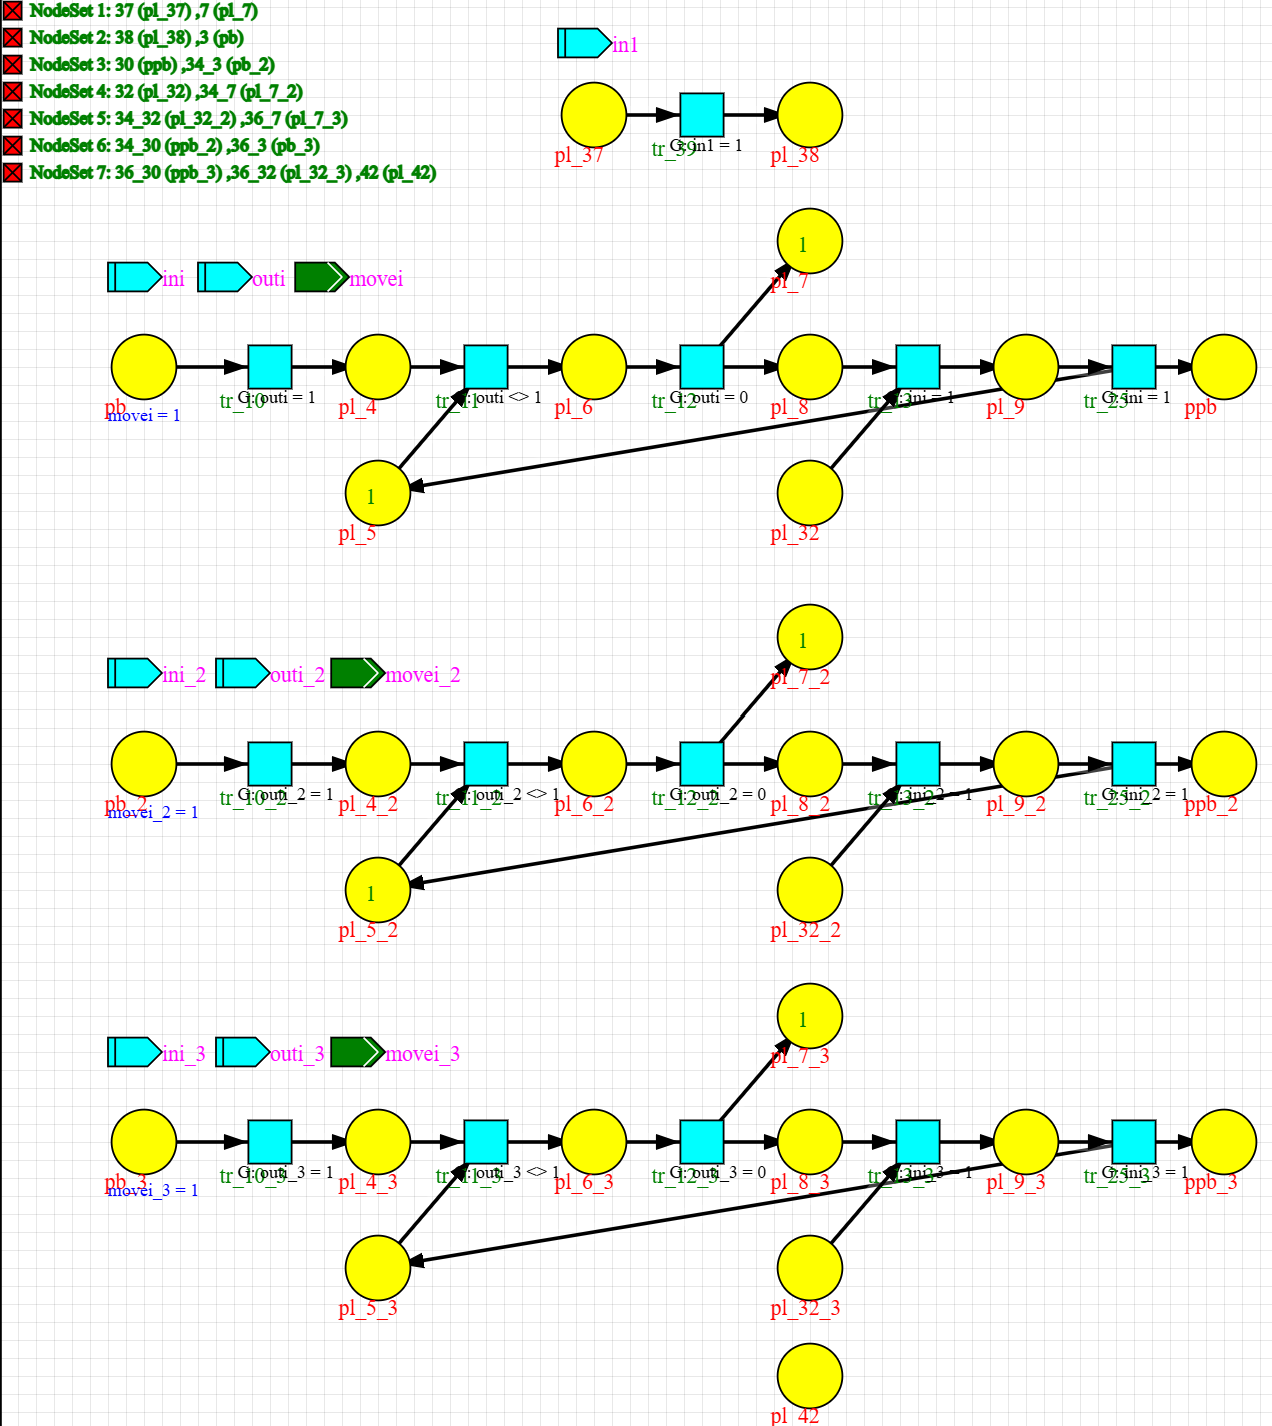
\includegraphics[width=0.8\textwidth]{img/petri_model_merge.png}
    \caption{Rede de Petri --- Fusion set}\label{fig:petri_fusion_set}
\end{figure}

\subsubsection{Rede de Petri --- Node set}
\begin{figure}[H]
    \centering
    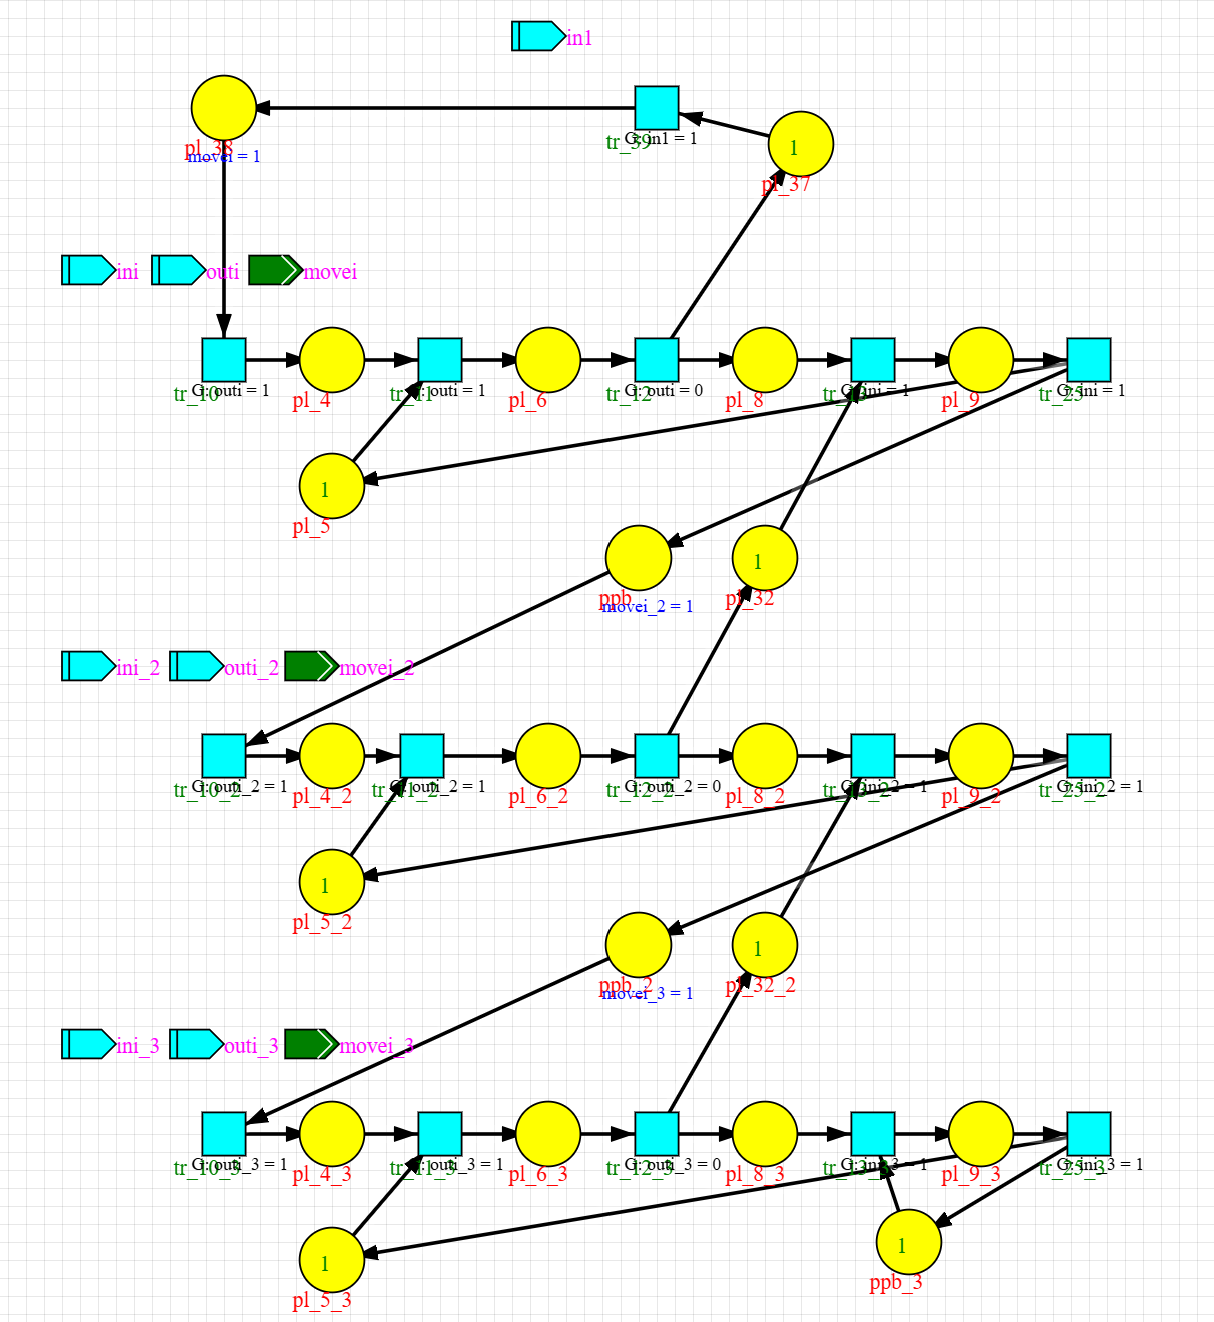
\includegraphics[width=0.8\textwidth]{img/petri_node_set.png}
    \caption{Rede de Petri - Node set}\label{fig:petri_node_set}
\end{figure}

\subsection{Simulação e Análise}

\subsubsection{Simulação com token-player}


Neste link tem acesso ao vídeo da simulação com token-player: 

\hspace{1em}

\url{https://unlpt-my.sharepoint.com/:v:/g/personal/jafe_lopes_fct_unl_pt/EUvkbe_KlbRFrrdI0gsSh98Bu2URieTdJFFzwphaj5HS6A?e=i5XMNg&nav=eyJyZWZlcnJhbEluZm8iOnsicmVmZXJyYWxBcHAiOiJTdHJlYW1XZWJBcHAiLCJyZWZlcnJhbFZpZXciOiJTaGFyZURpYWxvZy1MaW5rIiwicmVmZXJyYWxBcHBQbGF0Zm9ybSI6IldlYiIsInJlZmVycmFsTW9kZSI6InZpZXcifX0%3D}


\subsubsection{Simulação temporal}

\subsubsection{Geração e análise do espaço de estados}

\begin{figure}[H]
    \centering
    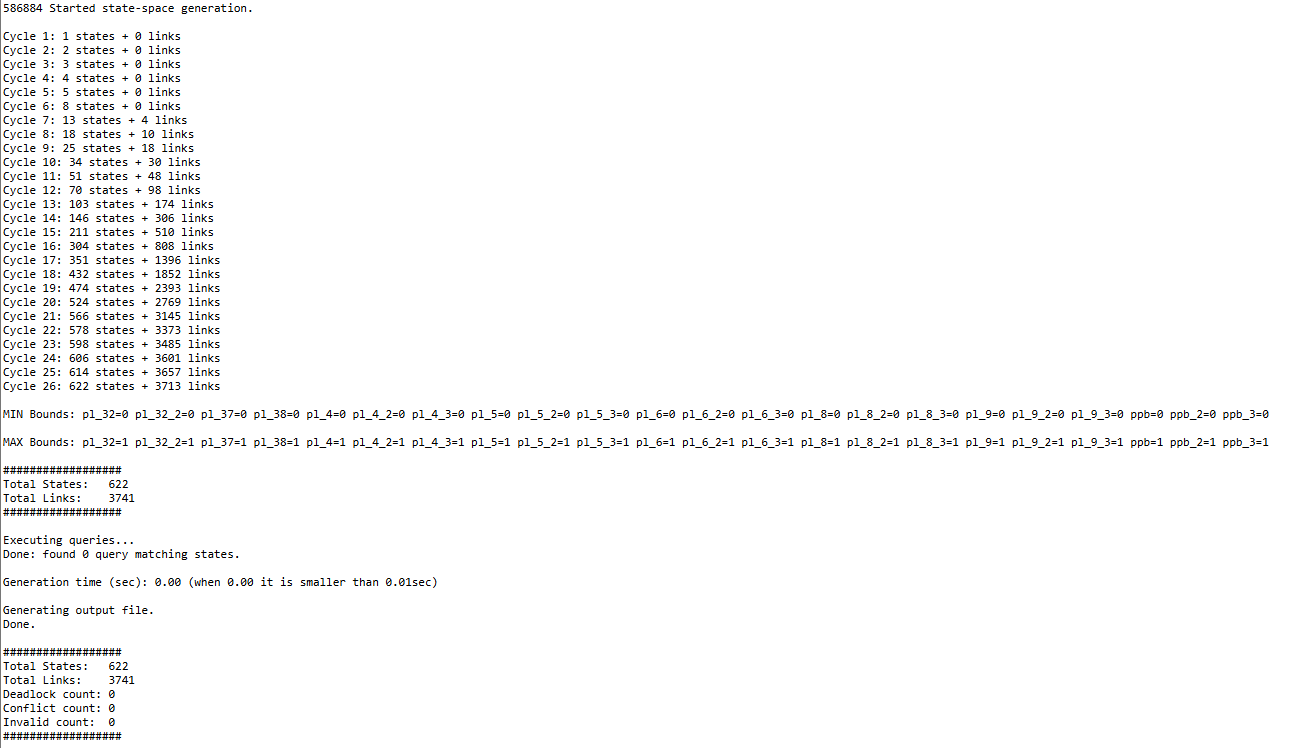
\includegraphics[width=1\textwidth]{img/petri_statespace.png}
    \caption{Rede de Petri --- Espaço de Estados}\label{fig:petri_statespace}
\end{figure}